\newcommand{\bY}{\mathbf{Y}}
\newcommand{\NN}{\mathbb{N}}         
%\nipsfinalcopy % Uncomment for camera-ready version

% \subsection{Notation}
% 
% Unless otherwise specified, we let lower-case English alphabet characters indicate scalars $x \in \Real$. Bold indicates column vectors $\mb{x} \in \Real^p$,
% and upper-case bold indicates matrices, $\bX \in \Real^{p \times q}$.  Parameters and constants are Greek characters.  Time is $t \in [0,T]$, 
% $i \in [N]$ indexes the $N$ neurons, where $[N]=\{1,2,\ldots,N\}$. Script denotes sets and pipes denote the cardinality of the set, e.g. $|\mc{T}|$.  We let $\equiv$ denote ``is shorthand for''. San serif fonts, e.g., $\mathsf{H}$, denote functions. 
% %\vspace{-.1in}
% \subsection{Input}
% %\vspace{-.1in}
% % \subsection{Data Model}
% Our data is a time-series of multielectrode recordings $\bX \equiv (\bx_1, \cdots, \bx_T)$, and consists of $T$ recordings from $M$ channels. 
% The set of recording times lie on regular grid with interval length $\Delta$, while $\bx(t) \equiv \bx_t\in \mathbb{R}^M$ for all $t$. 
% This time-series of electrical activity is driven by an unknown number of neurons;  
% we do not wish to bound this number \emph{a priori}. %, though only a few of the infinite
% =======
% \subsection{Data Model}

Our data is a time-series of multielectrode recordings $\bX \equiv (\bx_1, \cdots, \bx_T)$, and consists of $T$ recordings from $M$ channels. 
Underlying these recordings is a continuous-time voltage trace sampled on regular grid with interval length $\Delta$, while $\bx_t \in \mathbb{R}^M$ for all $t$. 
This electrical activity is driven by an unknown number of neurons, %and 
%we do not wish to bound this number \emph{a priori}. %, though only a few of the infinite
% >>>>>>> ff0f5b20cd09ef2d570aa2ed8ea5c6d04356249f
%neurons dominate. These neurons contribute the majority of the activity in any finite interval of time; however, as time passes, the total number of 
%observed neurons increases {\color{red}(Justify?)}. 
%Each neuron, has its own `shape' A natural model in such a situation is to
with the neurons themselves generating continuous-time voltage traces. 
The outputs of all neurons are superimposed and discretely sampled to produce the 
recordings $\bX$.  At a high level, we model the continuous-time output of each neuron as a
series of idealized Poisson events smoothed with appropriate kernels (the latter determining the shape of each spike).
We then provide a discrete-time approximation to this model based on the Bernoulli approximation to the Poisson process, and
apply this to the observed data.
%Each neuron has its own distribution over waveform shapes. 
% 
% We describe this in detail, starting first with a model for a single channel recording $\bx \equiv (x_1, \cdots, x_T)\T$.
% =======
We describe this below, starting first with a model for the continuous-time output $x(t)$ of a single neuron.
%channel recording $\bx\T \equiv (x_1, \cdots, x_T)$.
% >>>>>>> ff0f5b20cd09ef2d570aa2ed8ea5c6d04356249f

%\vspace{-.1in}
\subsection{Modeling a single electrode recording}
%\vspace{-.1in}

There is a rich literature characterizing the spiking activity of a single neuron \citep{?}, accounting in detail for factors like non-stationarity, 
refractoriness and spike waveform. We however make a number of simplifying assumptions (some of which we later relax).
%, others we leave for future work). 
Figure \ref{fig:schematic} \jovo{@dec - is this fig gonna happen?} provides a schematic depiction of our generative process.
First, we model the spiking activity of each neuron as stationary and memoryless, so that its set of spike times are 
distributed as a homogeneous Poisson process ($\mathsf{PP}$).  %{\color{red} justify?}
 We model the neurons themselves are heterogeneous, with the $i^{th}$ neuron having
an (unknown) firing rate $\lambda_i$. 
% For the $i^{th}$ neuron, the $j^{th}$ spike time is denoted $\tau_{ij} \in \mc{T}_i$
Call the ordered set of spike times of the $i^{th}$ neuron $\mc{T}_i=(\tau_{i1}, \tau_{i2},\ldots)$; then the time between successive elements of $\mc{T}_i$ is 
exponentially distributed with mean $1/\lambda_i$. We write this as
$ \mc{T}_i \sim \mathsf{PP}(\lambda_i)$.

The actual electrical output of a neuron is not binary; instead each spiking event is a smooth perturbation in voltage about a
resting state. This perturbation forms the shape of the spike, and without any loss of generality, we set the resting state to zero. 
%{(\color{red} figure? better biological description? comment on how we preprocess the data to get zero mean?)}. 
While the spike shapes vary across neurons as well as across different spikes of the same neuron, each 
neuron has its own characteristic distribution over shapes. 
We let $\bth^*_i \in \Theta$ parametrize this distribution for neuron $i$.
 % having parameter $\bth^*_i$. 
Whenever this neuron emits a 
spike, a new shape is drawn independently from the corresponding distribution. %$p_{\bth_i}$, and 
This waveform is then offset to the time of the spike, and contributes to the voltage trace associated with that spike. The complete recording from
the neuron is the superposition of all these spike waveforms plus noise.  
We start by assuming the noise at each observation time is i.i.d.\ Gaussian.

% Comment on how this dictionary is obtained now, or in section on inference?)}. 
We model the random spike shapes themselves as weighted superpositions of a dictionary of $K$ basis functions $\mathsf{\bd}(t) \equiv (\mathsf{d}_1(t), \cdots, \mathsf{d}_K(t))\T$. The
dictionary elements are shared across all neurons, and each is a real-valued function of time, e.g., $\mathsf{d}_k \in L_2$.
% For the $i^{th}$ neuron, the $j^{th}$ spike time $\tau_{ij} \in \mc{T}_i$, 
Each spike time $\tau_{ij}$ is associated with a random $K$-dimensional weight vector $\tby_{ij} \equiv (\ty_{ij1}, \ldots \ty_{ijK})\T$, and the 
shape of this spike at time $t$ is given by the weighted sum $\sum_{k=1}^K \ty_{ijk} \mathsf{d}_k(t-\tau_{ij})$. We assume $\tby_{ij} \sim \mathsf{N}_K(\mb{\mu}^*_i, \Sigma^*_i)$, indicating a $K$-dimensional 
Gaussian distribution with mean and covariance given by $(\mb{\mu}^*_i, \Sigma^*_i)$; we let $ \theta^*_i \equiv (\mb{\mu}^*_i, \Sigma^*_i) $.   Then, at any time $t$, the output of neuron $i$ is
$
  x_{i}(t) = \sum_{j=1}^{|\mc{T}_i|} \sum_{k=1}^K \ty_{ijk} \mathsf{d}_k(t - \tau_{ij}).
$

% 
% 
% 
% \begin{center}
% \begin{figure}
% % 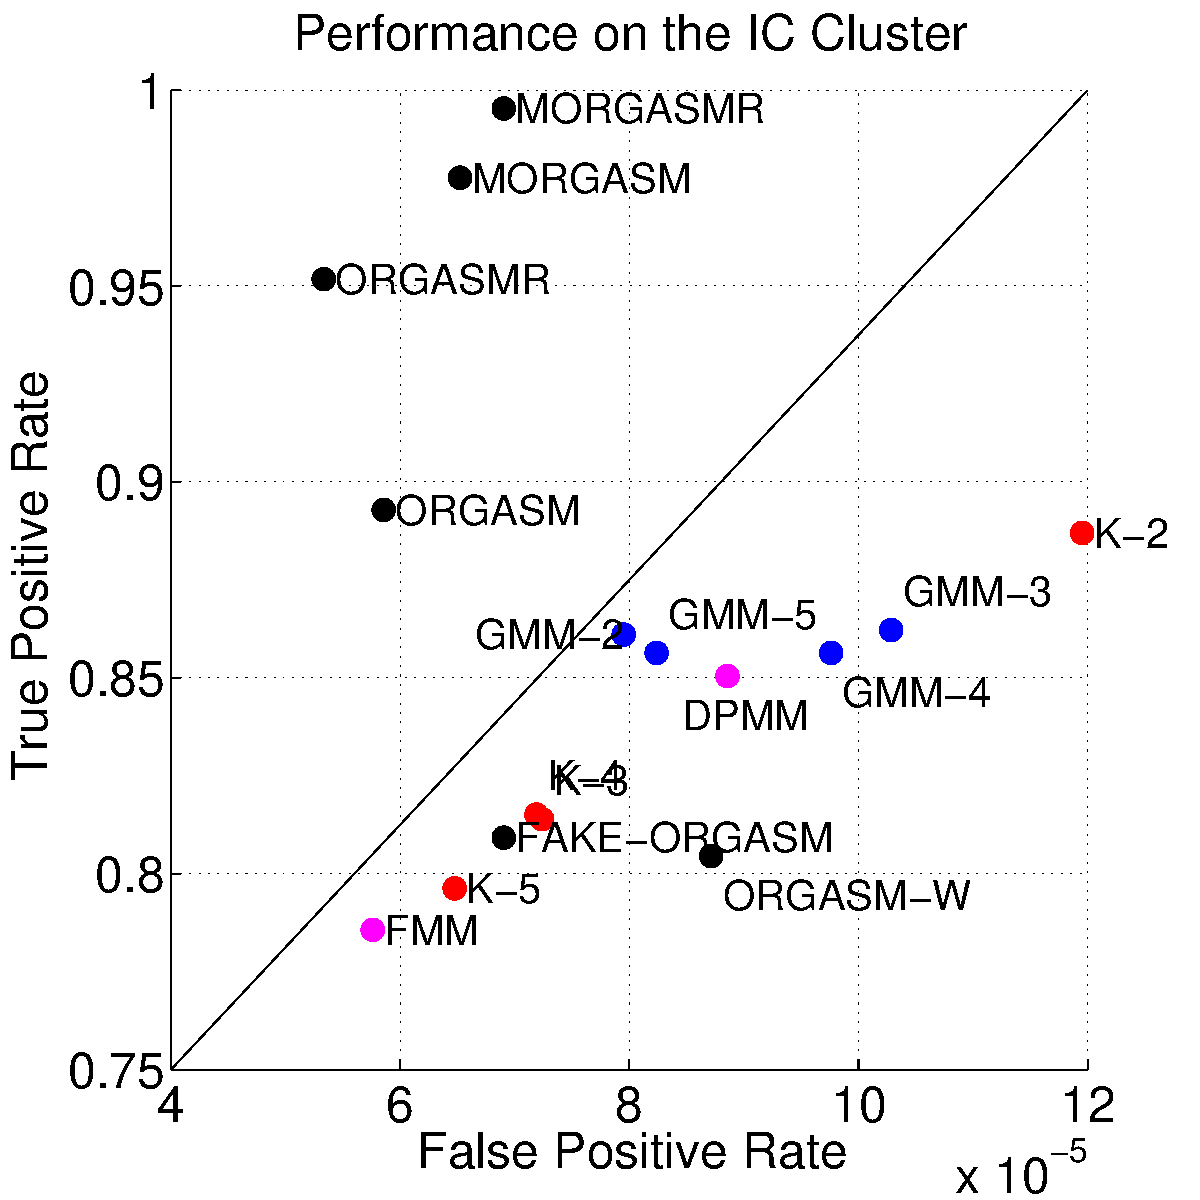
\includegraphics[width=\textwidth]{../figs/truefalsepositive}
% \caption{Schematic of our Generative Model.}
% \label{fig:schmetic}
% \end{figure}
% \end{center}
% 
{The total signal recorded from any electrode  is the superposition of the outputs of all neurons. Assume for the moment there are $N$
neurons, and define $\mc{T} \equiv \cup_{i \in [N]} \mc{T}_i$ as
the (ordered) union of the spike times of all neurons. 
Let $\tau_l \in \mc{T}$ indicate the time of $l^{th}$ overall spike, whereas $\tau_{ij} \in \mc{T}_i$ is the time of the $j^{th}$ spike of neuron $i$.
%To map elements  $\tau_{ij} \in \mc{T}_i$ to elements  $\tau_l \in \mc{T}$,   
This defines a pair of mappings: $\nu:[|\mc{T}|]\rightarrow [N]$, and $p:[|\mc{T}|]\rightarrow \mc{T}_{\nu_i}$, with %$(i = \nu(l))$, , which maps from the $j^{th}$ spikes of neuron $i$ to the $l^{th}$ overall spike.
$\tau_l = \tau_{\nu_l p_l}$. 
%\jovo{i don't think the square brackets around $\mc{T}$ are correct, we are mapping from the set of spikes, not the number of spikes, right?} 
In words, $\nu_l \in N$ is the neuron to which the $l^{th}$ element of $\mc{T}$ belongs, 
while $p_l$ indexes this spike in the spike train $\mc{T}_{\nu_l}$.
%\jovo{``position'' is weird to me.  can we say: ``indexes which spike of neuron $\nu_l$'', or something like that?}.
Let $\bth_l \equiv (\mb{\mu}_l, \Sigma_l)$ be the neuron parameter associated with spike $l$, so that $\bth_l = \bth^*_{\nu_l}$. 
Finally, define $\by_l \equiv (y_{l1}, \ldots, y_{lK})\T \equiv \tby_{\nu_j p_j}$ as the weight vector of spike $\tau_l$. Then, we have that}
% \begin{subequations}
\begin{align}
  x(t) &= \sum_{i \in [N]} x_{i}(t) =   \sum_{l \in |\mc{T}|} \sum_{k \in [K]} y_{lk} \mathsf{d}_k(t - \tau_{l}), \qquad %\label{eq:spk_sup} \\
% \intertext{where}
  \text{ where } \by_{l}  \sim \mathsf{N}_K(\mb{\mu}_{l}, \Sigma_{l}). \label{eq:spk}
\end{align}
% \end{subequations}
% 
From the superposition property of the Poisson process \citep{kingman93}, the overall spiking activity $\mc{T}$ is 
Poisson with rate $\Lambda = \sum_{i \in [N]} \lambda_i$. Each event $\tau_l \in \mc{T}$ has a pair of labels, its neuron parameter
$\bth_l \equiv (\mb{\mu}_l, \Sigma_l)$, and $\by_l$, the weight-vector characterizing the spike shape. We view these weight-vectors as the ``marks'' of a 
marked Poisson process $\mc{T}$.  From the properties of the Poisson process, we have that the marks $\bth_l$ are drawn i.i.d. from a probability measure:
$\quad  \mathsf{G}(\dd \bth) = 1/\Lambda\sum_{i \in [N]} \lambda_i \delta_{\bth^*_i}$.
\vspace{-.27in}
\begin{align}
    \label{eq:mark_distr}
\end{align}
Note that with probability one, the neurons have distinct parameters, so that the mark $\bth_l$ associated with spike $l$ identifies the
neuron which produced it: $\mathsf{G}(\bth_l = \bth^*_i) = \mathsf{P}(\nu_l= i) = \lambda_i/$$\Lambda$. Given $\bth_l$, $\by_l$ is distributed as in
Eq.~\eqref{eq:spk}. The output waveform $x(t)$ is then a linear functional of this marked Poisson process. % (Eq.~\eqref{eq:spk_sup}). 

%\vspace{-.1in}
\subsection{Completely random measures (CRMs)}
%\vspace{-.1in}

%The previous section assumed a known number of neurons $N$; 
In practice, our recordings are a superposition of outputs of an unknown
number of neurons. We do not wish to bound this number \emph{a priori}, moreover we expect this number to increase as we 
record over longer intervals. This suggests a nonparametric Bayesian approach: allow the \emph{total} 
number of underlying neurons to be infinite.
Since only a finite number of spikes are observed in any finite interval, only a finite number of neurons will be \emph{active}.
Onlt a few neurons dominate spiking activity over any interval (the complexity of the
data will suggest how many).
This elegant and flexible modeling approach has  already proved 
successful in neuroscience applications \citep{WoodBla2008}.
%where we allow the number of neurons to be infinite.
%this leads to 
%While the number of neurons observed over any finite observation interval is finite, this number increases with the observation interval. 
%This makes sense in a biological context, in that as we record for longer (e.g., days, weeks, or months even), certain neurons will die or drop-out, and others will appear, simply by virtue of the electrodes moving, for example. 
 %, moreover the total rate $\Lambda$ of all neurons must also be finite.
%the total rate $\Lambda$ must 
%also be finite. Moreover, we want this to be dominated by a few $\lambda_i$: the corresponding neurons contribute the majority of the spiking
%activity in the observation interval. 

% A natural framework that captures our  modeling requirements is that of \emph{completely random measures} (CRMs) \citep{Kingman:PJM67}.
% CRMs are stochastic processes that form flexible and convenient priors over
% infinite dimensional objects like probability distributions \citep{JamesLP09}, hazard functions \citep{Hjo1990}, latent features \citep{ThiJor2007}. 
% These have been well studied in the Bayesian nonparametrics and machine learning communities, and there is a wealth of literature on
% theoretical properties, as well as posterior computation.
% 
% Recall that each neuron is characterized by a pair of parameters $(\lambda_i, \bth^*_i)$; characterizing the distribution over spike times 
% and shapes respectively. With Eq.~\eqref{eq:mark_distr} in mind, we map the infinite collection of pairs $\{(\lambda_i, \bth^*_i)\}$ to an atomic measure on $\Theta$:
% $\quad \mathsf{\Lambda}(\dd \bth) = \sum_{i=1}^{\infty} \lambda_i \delta_{\bth^*_i}$.
% 
% =======
A natural framework for our requirements is that of \emph{completely random measures} (CRMs) \citep{Kingman:PJM67}.
%CRMs are stochastic processes that form flexible and convenient priors over
%infinite dimensional objects like probability distributions \citep{JamesLP09}, hazard functions \citep{Hjo1990}, latent features \citep{ThiJor2007}. 
CRMs have been well studied in the Bayesian nonparametrics community, and there is a wealth of literature on
theoretical properties, as well as posterior computation; see \citep{JamesLP09, Hjo1990, ThiJor2007} for example. 
%Recall that each neuron is characterized by a pair of parameters $(\lambda_i, \bth^*_i)$; characterizing the distribution over spike times 
%and shapes respectively. 
With Eq.~\eqref{eq:mark_distr} in mind, and recalling that each neuron is characterized by a pair of parameters $(\lambda_i, \bth^*_i)$,
we map the infinite collection of pairs $\{(\lambda_i, \bth^*_i)\}$ to an atomic measure on $\Theta$:
$\ \  \Lambda(\dd \bth) = \sum_{i=1}^{\infty} \lambda_i \delta_{\bth^*_i}$.
% >>>>>>> ff0f5b20cd09ef2d570aa2ed8ea5c6d04356249f

For a CRM, the distribution over measures is induced by distributions
over the infinite sequence of weights, and the infinite sequence of their locations. 
The weights $\lambda_i$ are the jumps of a \Levy process \citep{Sato90}, and their distribution is characterized by a 
\Levy measure $\rho(\lambda)$. The locations $\bth^*_i$ are drawn i.i.d.\  from a base probability measure $H(\bth^*)$.
As is typical, we assume these to be independent. % (though this is not necessary). 
%{\color{green} if there's space, I
%can elaborate on the construction of the CRM from its Levy measure, though this is not necessary}

We set the \Levy measure $\rho(\lambda) = \alpha \lambda^{-1}\exp(-\lambda)$,
resulting in a CRM called the Gamma process ($\Gamma$P) \citep{applebaum2004}. 
The Gamma process has the convenient property that the 
total rate $\Lambda \equiv \mathsf{\Lambda}(\Theta) = \sum_{i=1}^{\infty} \lambda_i$ is Gamma distributed (and thus conjugate to the Poisson process prior on $\mc{T}$).
%\footnote{We abuse notation by using $\Lambda$ to denote both the measure as well as the total measure of $\Theta}
%The Gamma distribution has shape parameter $1$ and scale parameter $\alpha$.  Since this is finite almost surely, so too is $\mc{T}$. 
The Gamma process is also closely connected with the Dirichlet process \citep{Ferguson73}, which will prove useful
later on.
Other choices of the \Levy intensity can be used to capture greater uncertainty in the number of neurons active in any finite interval, or to model
power-law behavior in the number of spikes emitted by different neurons.

% To complete the specification on the Gamma process, we choose a base-measure $\mathsf{H}(\bth^*)$.
% %Recalling that $\bth^* \equiv (\mu^*, \Sigma^*)$ gives the mean and variance of the weight-vector $\by^*$ of a neuron, 
% We set $\mathsf{H}(\bth^*)$ 
% to the conjugate normal-Wishart distribution with parameters $\phi$. 
% =======
To complete the specification on the Gamma process, %we choose a base-measure $H(\bth^*)$.
%Recalling that $\bth^* \equiv (\mu^*, \Sigma^*)$ gives the mean and variance of the weight-vector $\by^*$ of a neuron, 
we set $H(\bth^*)$ 
to the conjugate normal-Wishart distribution with hyperparameters $\phi$.
% >>>>>>> ff0f5b20cd09ef2d570aa2ed8ea5c6d04356249f
%Our overall model is then:
%\begin{subequations}
%\begin{align}
%  \mc{T}_i\ \  &\sim \mathsf{PP}(\lambda_i) \quad i \in \NN, \quad &\text{ where } \mathsf{\Lambda}(\cdot)&=\sum_{i=1}^{\infty} \lambda_i \delta_{\theta^*_i} \sim \Gamma \text{P}(\alpha, \mathsf{H}(\cdot| {\phi})), \\ %\mathcal{NW}(\mu, \Sigma)) \\ \\
%\vspace{-.8in}
%  x_i(t) &= \sum_{j = 1}^{|\mc{T}_i|}  \sum_{k = 1}^{K} y^*_{ijk} \mathsf{d}_k(t - \tau_{ij}), \quad &\text{ where }\by^*_{ij}  &\sim \mathsf{N}_K(\mb{\mu}^*_i, \Sigma^*_i) \quad i,j \in \NN, \\
%  x(t)   &= \sum_{i=1}^{\infty} x_i(t) + \eps_t, \quad &\text{ where at any time $t$, } \eps_t &\sim \mathsf{N}(0,\Sigma_x) \text{ independently}
%\end{align}
%\end{subequations}

%Each spike of each neuron is associated with a time $e$ and a weight vector $y$, and one can view the model above as a doubly stochastic Poisson
%process on the product space. 
% 
%\jovo{perhaps it is standard, but you sample $\Lambda$ and then the next line you have $\lambda_i$, but no explanation for how you from $\Lambda$ to $\lambda_i$. i also am confused as to why $\phi$ is a subscript on $H$, rather than in the $(\cdot)$}
%Atom $i$ of the CRM corresponds to a neuron with parameters $(\lambda_i, \theta^*_i)$. 
It is easy to directly specify the resulting continuous-time model, we provide the equations in the Supplementary material. 
However it is more convenient to rerepresent the model using the marked Poisson process of Eq.~\eqref{eq:spk}. % and \eqref{eq:spk_shape}. 
The overall process $\mc{T}$ is a rate $\Lambda$ Poisson process,
and under a Gamma process prior, $\Lambda$ has a Gamma$(\alpha,1)$ distribution %with shape and scale parameters $\alpha$ and $1$ respectively 
\citep{Ferguson73}.
As we saw (Eq.~\eqref{eq:mark_distr}), the labels $\bth_i$ assigning events to neurons are drawn i.i.d. from a normalized Gamma 
process: % $\mathsf{G}(\dd \bth)$:
%\vspace{-.2in}
%\begin{align}
$ \mathsf{G}(\dd \bth) = \frac{1}{\Lambda} \sum_{l=1}^{\infty} \lambda_l$.
%\end{align}

$\mathsf{G}(\dd \bth)$ is a random probability measure called a \emph{normalized random measure} \citep{JamesLP09}. Crucially, a 
normalized Gamma process is the Dirichlet process (DP) \citep{Ferguson73}, so that $G$ is a draw from a Dirichlet process. For the $l^{th}$ spike in $\mc{T}$, given its 
parameter $\bth_l$, its shape vector is drawn from a normal distribution
with parameters $(\mb{\mu}_{l}, \Sigma_{l})$. Thus the spike parameters $\bth$ are i.i.d.\ draws from a Dirichlet process, while the weight vectors are
draws from a DP mixture model (DPMM) of Gaussians \citep{Lo1984}.

% <<<<<<< HEAD
% The connection with the DP allows us to simplify the representation of our model. In particular, we exploit a remarkable property of the DP that
% allows us to integrate out the infinite-dimensional variable $\mathsf{G}(\cdot)$. The resulting marginal distribution over observations follows the so-called
%  Chinese restaurant process ($\mathsf{CRP}$) \citep{Pit2002a}. Under this scheme, the $l^{th}$ spike is assigned the same parameter as an earlier spike with probability 
% =======
%The connection with the DP allows us to simplify the representation of our model. In particular, 
We can exploit the connection with the DP to %a remarkable property of the DP that allows us to 
integrate out the infinite-dimensional measure $G(\cdot)$ (and thus $\Lambda(\cdot)$), and assign spikes to neurons via 
%. The resulting marginal distribution over observations follows 
the so-called Chinese restaurant process (CRP) \citep{Pit2002a}. Under this scheme, the $l^{th}$ spike is assigned the same parameter as an earlier spike with probability 
% >>>>>>> ff0f5b20cd09ef2d570aa2ed8ea5c6d04356249f
proportional to the number of earlier spikes having that parameter. It is assigned a new parameter (and thus, a new neuron is observed) with probability 
proportional to $\alpha$. Letting $C_t$ be the number of neurons observed until time $t$, and  $\mc{T}^t_i = \mc{T}_i \cap [0,t)$ be the times of spikes 
produced by neuron $i$ before time $t$,
we then have for spike $l$ at time $t = \tau_l$: 
\vspace{-.06in}
\begin{align}
  P({\nu_l} = i) & \propto 
  \begin{cases}
   |\mc{T}^t_i| \quad i \in \{1,\cdots, C_{t}\}, \\
   \alpha \quad\ i = C_{t} + 1, 
  \end{cases}  
\label{eq:crp_marg_pr}
\end{align}
%\footnote{Strictly speaking, the process we just described is called a P\'olya urn scheme \citep{BlaMac1973}; for simplicity, we do not distinguish between this and the \mathsf{CRP}.}.
and $\bth_l = \bth^*_{\nu_l}$. 
This marginalization property of the DP allows us to integrate out the infinite-dimensional rate vector $\mathsf{\Lambda}(\cdot)$, and sequentially 
assign spikes to neurons based on the assignments of earlier spikes.
%is assigned (or equivalently, the parameter $\bth$ associated with that neuron). These marks are drawn from a probability measure 
%$\mathsf{G}(\dd \bth) = \frac{1}{R} R(\dd \bth)$. From the properties of the Gamma process, the probability measure $G$ a Dirichlet process, 
Doing so requires one final property: for the Gamma process, the random probability measure $\mathsf{G}(\cdot)$ is independent of the total mass $\Lambda$. 
Consequently, the clustering of spikes (determined by $\mathsf{G}(\cdot)$) is independent of the rate $\Lambda$ at which they are produced. We then have
 the following model equivalent to the one above:
\begin{subequations}
\begin{align}
  \mc{T} &\sim \mathsf{PP}(\Lambda), \qquad &\text{ where } \Lambda  &\sim \mathsf{\Gamma P}(\alpha, 1),
   \\
  \by_l &\sim \mathsf{N}_K(\mb{\mu}_{l}, \Sigma_{l}), \qquad &\text{ where } (\mb{\mu}_{l}, \Sigma_{l})  &\sim {\mathsf{CRP}}(\alpha, \mathsf{H}_{\phi}(\cdot)), \quad  l \in [|\mc{T}|],   \label{eq:CRP}\\
   % (\mb{\mu}_{l}, \Sigma_{l}) &\equiv \bth_l,  &\text{ where } \bth_l &\sim \text{\mathsf{CRP}}(\alpha, \mathsf{H}_{\phi}(\cdot)), \quad l \in [|\mc{T}|],   \label{eq:\mathsf{CRP}}\\
  x(t) &=   \textstyle{\sum_{l \in |\mc{T}|}} \sum_{k \in [K]} y_{lk} \mathsf{d}_k(t - \tau_{l}) + \eps_t  &\text{ where }  \eps_t &\iid \mathsf{N}(0,\sigma^2),  \,  l \in [|\mc{T}|].   \label{eq:CRP_mix}
\end{align} \label{eq:marked_pp}
\end{subequations}
% Unlike most applications which observe the outputs of a $\mathsf{CRP}$, our observation at any time $t$ is a convolution-like function of the $\mathsf{CRP}$ outputs of all
% earlier times. Consequently, we cannot directly apply standard techniques for posterior inference. In \S \ref{sec:inf}, we develop a novel online 
% algorithm for posterior inference; first, we provide a discrete-time approximation to our model.
% =======
%Unlike most applications which observe the outputs of a CRP, our observation at any time $t$ is a convolution-like function of the CRP outputs of all
%earlier times. Consequently, we cannot directly apply standard techniques for posterior inference. In \S \ref{sec:inf}, we develop a novel online 
%algorithm for posterior inference; first, we provide a discrete-time approximation to our model.
% >>>>>>> ff0f5b20cd09ef2d570aa2ed8ea5c6d04356249f

%For neuron $i$, the sequence of spike times is distributed as a Poisson process with random rate $\lambda_i$.
%Each event $\tau_{ij}$ is associated with a mark or label $y_{ij}$ drawn from a normal distribution (again, with random parameters).
%More broadly, we can view the superposed process $\mc{T}$ as a rate $\Lambda$ Poisson process, with each event having a pair of marks, the neuron identity $i$,
%and weight $y$. From the properties of the Gamma process, the pair form a draw from a Dirichlet process.
%Our data is in a form that makes discrete-time modeling more natural, and an approach now is
%one based on the Beta process-binomial process.

%\vspace{-.1in}
% =======
\vspace{-.2in}
% >>>>>>> ff0f5b20cd09ef2d570aa2ed8ea5c6d04356249f
\subsection{A discrete-time approximation}
\vspace{-.1in}
The previous subsections modeled the continuous-time voltage output of a neuron. Our data on the other hand consists of recordings
at a discrete set of times. While it is possible to make inferences about the continuous-time process underlying these discrete recordings,
in this paper, %for simplicity, 
we restrict ourselves to the discrete case. %We thus provide a discrete-time approximation to the model above. 
The marked Poisson process characterization of Eq.\ \ref{eq:marked_pp} leads to a simple
discrete-time approximation of our model.

Recall first the Bernoulli approximation to the Poisson process: a sample from a Poisson process with rate $\Lambda$ can be approximated by discretizing
time at a granularity $\Delta$, and assigning each bin an event independently with probability $\Lambda\Delta$ (the accuracy of the approximation increasing 
as $\Delta$ tends to $0$).
%
%This suggests the following approximation at a time resolution $\Delta$. Draw the random Poisson process rate $\Lambda$ drawn from a Gamma$(1,\alpha)$ 
%distribution. Simultaneously, draw a random probability measure
% $G$ from a Dirichlet process. Assign an event to an interval independently with probability $\Lambda\Delta$, and to each event, assign a random mark drawn 
To approximate the \emph{marked} Poisson process $\mc{T}$, all that is additionally required is to assign marks $\bth_i$ and $\by_i$ to each event 
in the Bernoulli approximation. Following Eqs.~\eqref{eq:CRP} and \eqref{eq:CRP_mix}, the $\bth_l$'s are distributed according
to a Chinese restaurant process, while each $\by_l$ is drawn from a normal distribution parametrized by the corresponding $\bth_l$. We discretize the 
elements of dictionary $\mathsf{d}_k \equiv \{\mathsf{d}_k(t)\}_{t \in (0,T)}$ as well, %defining a mapping from $L_2$ to $\Real^L$ 
yielding discrete dictionary elements 
$\mt{\bd}_{k,:}=(\mt{d}_k[1], \ldots, \mt{d}_k[L])\T$. These form the rows of a ${K \times L}$ matrix $\mt{\bD}$ (we call its columns
$\mt{\bd}_{:,h}$). The shape of the $j^{th}$ spike is now a vector of length $L$, and for a weight vector
$\by$, is given by $\mt{\bD} \by$.

We can simplify notation a little for the discrete-time model. Let $t$ index time-bins (so that for an observation interval of length 
$T$, $t \in [T/\Delta]$).
Let the binary variable $\mt{z}_t$ indicate whether or not a spike in present in time bin $t$ (recall that 
$\mt{z}_t \sim \text{Bernoulli}(\Lambda \Delta)$). Let
$\mt{\nu}_t$ and $\mt{\theta}_t$ be the neuron and neuron parameter associate with time bin $t$, and let $\mt{\by}_t$ be its weight-vector. 
If there is a spike associated with that bin (i.e.\ 
$\mt{z}_t = 1$), then these are the marks of that spike, otherwise we ignore them.
Then the output at time $t$, $x_t$ is given by
%\begin{align}
$\quad  x_t = \sum_{h = 1}^L \mt{z}_{t-h} \mathsf{\bd}_{:,h}^{\T} \mt{\by}_{t-h-1} + \eps_t \text{,\quad where $\eps_t \iid \mathsf{N}(0,\sigma^2)$.}$ 
%\end{align}
\vspace{-.1in}
\subsection{Correlations in time and across electrodes}
\vspace{-.1in}
We end by describing some extensions to the model outlined so far. 
%The first is the inclusion of measurement noise: {\color{red} Biology?}. Let $\eps_t$ be the noise at time $t$, we model this as independent, additive and Gaussian.
%However, rather than modeling the noise as independent across time, we model it as a first-order autoregressive process. This can capture
%effects like the movement of electrodes during the experiment. 
The first relaxes the requirement that the parameters $\bth^*$ of each neuron remain constant, instead allowing $\mb{\mu}^*$, the mean of the weight-vector,
to evolve with time (we keep the covariance parameter $\mb{\Sigma}^*_i$ fixed, however). Such flexibility can capture effects like changing cell 
characteristics or moving electrodes.
We model the time-evolution of the mean vector of a neuron as a realization of a Gaussian process (GP) \citep{RasWil2006}. A consequence is that the 
means remain marginally Gaussian distributed at any time, on the other hand correlation between means across time is determined by the choice 
of the GP covariance kernel.
We choose a stationary Markov kernel (where covariance decays exponentially with time); in discrete-time, this corresponds to a simple first-order 
autoregressive process. With $\mb{A} \in \mathbb{R}^{K \times K}$ the transition matrix, and $\mb{r}_t \in \mathbb{R}^K$, 
independent and Gaussian {innovations}, we have

% \begin{align}
  $\mb{\mu}^*_{t+1} = \mathbf{B} \mb{\mu}^*_t + \mathbf{r}_t$.
% \end{align}
Where we previously had a DP mixture of Gaussians, we now have a DP mixture of GPs. Each neuron is now associated with a vector-valued function 
$\bth^*(\cdot)$, rather than a constant. When a spike at time $\tau_l$ is assigned to neuron $i$, it is assigned a weight-vector $\by_l$ drawn from a 
Gaussian with mean $\mb{\mu}^*_i(\tau_l)$. %Following \citep{wood2009}, a useful extension is to also allow the neuron assignment probabilities to evolve 
%(corresponding to a time-varying Gamma process \citep{RaoTeh2009a}); we leave this for future work. 
In a similar way, we also induce correlations in the noise, we model this as an AR process with transition matrix $\mathbf{B}$.

Our second extension is to generalize our model from a single electrode to the case of multielectrode recordings. 
We allow the shape of any spike to vary across channels: for spike $l$ in channel $m$, call the weight-vector $\by^m_l$.
Of course, all these vectors need to be correlated as they correspond to the same spike. We do this simply by concatenating the set of vectors into
a single $MK$-element vector $\by_l = (\by^1_l;\cdots;\by^M_l)$, and modeling this as a multivariate normal. In principle, one might expect the associated 
covariance matrix to possess a block structure (corresponding to subvector associated with each channel); however, rather than building this into the model,
we allow the data to inform us about any such structure.
Algorithm \ref{alg:gen_proc} in the supplementary material outlines generative mechanism of the data for the discrete-time model.

